\documentclass[11pt]{article}

\usepackage[margin=1in]{geometry}
\usepackage{amsmath,amssymb}
\usepackage{graphicx}
\usepackage{booktabs}
\usepackage{tikz}
\usepackage{xcolor}
\usepackage{hyperref}
\usepackage{natbib}
\usepackage{caption}
\usetikzlibrary{arrows.meta, positioning}

\hypersetup{colorlinks=true, linkcolor=blue, citecolor=blue, urlcolor=blue}

\title{\textbf{OctoLoRA: Gradient-Adaptive Rebalancing of LoRA+ \\ for Low-Rank Fine-Tuning}}
\author{
  Fabio Ciraci \\
  \small University of Bologna, DISI \\
  \small \texttt{fabio.ciraci@unibo.it}
}
\date{}

\begin{document}
\maketitle

\begin{abstract}
Low-Rank Adaptation (LoRA) trains a small update $B A$ on top of a frozen
weight matrix, but $A$ and $B$ do not train at compatible rates: $B$'s
zero initialization leaves it undertrained relative to $A$ under a shared
learning rate. LoRA+ fixes this with a fixed learning-rate ratio between
the two matrices. We introduce a simple, training-time-only modification —
a per-layer gate that rescales the gradient reaching $A$ based on an
exponential moving average of $A$'s and $B$'s recent gradient norms —
intended to make that ratio adaptive rather than fixed. The gate never
changes the forward computation, so it adds zero inference cost and zero
parameters. On GSM8K with Llama-3.1-8B-Instruct, we find the method's
naive evaluation is misleading: at LoRA+'s commonly-cited default ratio
(16), our combined method \emph{loses} to plain LoRA by 3.8 percentage
points, and this initially looked like the method didn't work at all.
Diagnosing training loss against test accuracy revealed the LoRA+ variants
were overfitting; sweeping the ratio down to 2 recovers and then exceeds
plain LoRA's performance. At this corrected ratio, gate $+$ LoRA+ beats
plain LoRA by 1.3 percentage points on average, confirmed across three
seeds with non-overlapping accuracy ranges. We report this result together
with its full negative-result history, situate it against more principled
recent fixes for the same A/B-imbalance problem (LoRA-RITE, ALLoRA) whose
reported effect sizes are substantially larger, and are explicit about the
narrow, hyperparameter-sensitive scope of what we show.
\end{abstract}

\section{Introduction}

Fine-tuning large language models by updating every parameter is
expensive. LoRA \citep{hu2021lora} makes this cheap: freeze a pretrained
weight matrix $W$, and learn a low-rank update $\Delta W = BA$, where
$A \in \mathbb{R}^{r \times d_{in}}$ and $B \in \mathbb{R}^{d_{out} \times
r}$ with rank $r \ll \min(d_{in}, d_{out})$. Only $A$ and $B$ are trained.

A known inefficiency in this recipe is that $A$ and $B$ do not train at
compatible rates. $A$ is randomly initialized and $B$ is initialized to
zero, and \citet{hayou2024lora} show that under a shared learning rate this
asymmetry causes $B$ to be systematically undertrained as model width
grows. Their fix, \textbf{LoRA+}, is a single global hyperparameter: give
$B$ a fixed learning-rate multiplier (16$\times$ by default) relative to
$A$, for the entire training run.

This paper investigates a natural follow-up question: if a \emph{fixed}
ratio helps, does an \emph{adaptive} one help more? We implement a
per-layer gate that tracks an exponential moving average (EMA) of the
gradient norms flowing into $A$ and $B$ separately, and uses their ratio
to rescale how much of $A$'s gradient is allowed through at each training
step — a dynamic, per-layer analogue of LoRA+'s fixed, global ratio. We
call the resulting method \textbf{OctoLoRA}.

The empirical path to our result is unusually informative and we report it
in full rather than only the final number. An initial ablation at LoRA+'s
default ratio (16) showed the combined method losing to plain LoRA by
3.8 points — the opposite of our hypothesis. Rather than treat this as a
negative result, we diagnosed it: comparing training loss to test accuracy
showed the LoRA+ variants were \emph{overfitting}, and sweeping the ratio
down revealed a clear, monotonic recovery. At a corrected ratio of 2, the
full method beats plain LoRA by 1.3 points on average, confirmed across
three random seeds with non-overlapping accuracy ranges. We consider this
progression — wrong hyperparameter, apparent negative result, correct
diagnosis, corrected and confirmed positive result — as important to the
paper's contribution as the final number, since it is a directly
reproducible cautionary tale about drawing conclusions from a single,
unswept hyperparameter setting.

We make three contributions:
\begin{enumerate}
  \item A gradient-adaptive, per-layer alternative to LoRA+'s fixed
  learning-rate ratio, requiring no additional parameters and no change to
  the forward computation (Section~\ref{sec:method}).
  \item An empirical demonstration on GSM8K fine-tuning of
  Llama-3.1-8B-Instruct that the method's apparent failure at a commonly
  used hyperparameter setting is an artifact of that setting, not of the
  method, and that a corrected setting yields a real, seed-confirmed
  improvement (Section~\ref{sec:results}).
  \item A comparison against concurrent, more principled solutions to the
  same problem (LoRA-RITE, ALLoRA) that situates our effect size honestly
  relative to the current state of the art, rather than only against LoRA
  and LoRA+ (Section~\ref{sec:related}).
\end{enumerate}

\section{Related Work}
\label{sec:related}

\paragraph{LoRA and LoRA+.} LoRA \citep{hu2021lora} is the foundation this
work builds on. LoRA+ \citep{hayou2024lora} is the method we directly
modify: a fixed, global learning-rate ratio between $A$ and $B$, motivated
by a width-scaling analysis of feature learning. It is the correct
baseline for our ablation, since our gate targets exactly the imbalance
LoRA+ targets, only adaptively.

\paragraph{Other adaptive fixes for the A/B imbalance.} We are not the
only recent attempt to make this fix adaptive rather than fixed.
\textbf{ALLoRA} \citep{allora2024} scales per-row gradients inversely
proportional to the $\ell_2$ norm of that row of $BA$, an instantaneous
(no-EMA) weight-magnitude-driven rule; it reports a modest but consistent
average improvement (+0.3\%) over LoRA and DoRA across several models.
\textbf{LoRA-RITE} \citep{lorarite2024} addresses a related but distinct
issue — transformation invariance, the fact that many $(A,B)$ pairs
represent the same product $BA$ with very different condition numbers —
via optimizer-level matrix preconditioning derived from a polar
decomposition. It is a substantially more principled and expensive
method than ours, and reports large, verified gains: +7.13 points on
GSM8K (Gemma-7B, 48.37\%~$\to$~55.50\% over plain Adam) and +8.2 points
on a broader benchmark average. \textbf{Balanced LoRA (BaLoRA)}
\citep{balora2026} takes a third angle, projecting $(A,B)$ onto a
manifold that improves the pair's condition number each step; its
abstract claims faster convergence and superior performance but we could
not verify specific benchmark numbers from the available text. None of
these three methods use our specific construction (an EMA of gradient
norms as a scalar gate on gradient flow into $A$), but the problem space
is considerably more active and, in LoRA-RITE's case, considerably
better-solved than a comparison against LoRA+ alone would suggest — we
return to this in Section~\ref{sec:discussion}.

\paragraph{FlyLoRA and the multi-task interference problem.} FlyLoRA
\citep{flylora2025} is a different problem behind a similar name: it
addresses \emph{inter-task} interference when multiple LoRA adapters are
merged, using a frozen random sparse projection (inspired by the fly
olfactory circuit) in place of a trainable down-projection, together with
rank-wise expert activation in the up-projection — an implicit
Mixture-of-Experts with no trainable router. Our method has no expert
routing, no multi-adapter merging setting, and targets single-task
training dynamics, not cross-task interference. We note this explicitly
because our project's working name was inspired by FlyLoRA's biological
framing; the two methods are otherwise unrelated, and FlyLoRA is not a
directly competing baseline for what we evaluate here.

\section{Method}
\label{sec:method}

\begin{figure}[t]
\centering
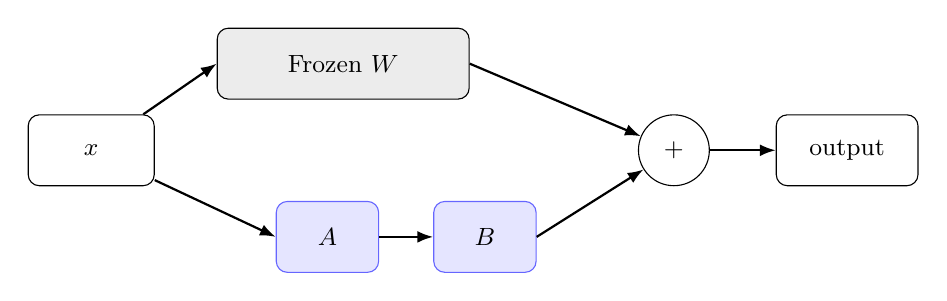
\begin{tikzpicture}[
  box/.style={draw, rounded corners, minimum height=0.9cm, align=center, font=\small},
  frozenbox/.style={box, fill=gray!15},
  adaptbox/.style={box, fill=blue!10, draw=blue!60},
  arr/.style={-{Latex[length=2mm]}, thick}
]
  \node[box, minimum width=1.6cm] (x) at (0,0) {$x$};
  \node[frozenbox, minimum width=3.2cm] (W) at (3.2,1.1) {Frozen $W$};
  \node[adaptbox, minimum width=1.3cm] (A) at (3.0,-1.1) {$A$};
  \node[adaptbox, minimum width=1.3cm] (B) at (5.0,-1.1) {$B$};
  \node[box, minimum width=0.7cm, circle] (sum) at (7.4,0) {$+$};
  \node[box, minimum width=1.8cm] (out) at (9.6,0) {output};

  \draw[arr] (x) -- (W.west);
  \draw[arr] (x) -- (A.west);
  \draw[arr] (A) -- (B);
  \draw[arr] (W.east) -- (sum);
  \draw[arr] (B.east) -- (sum);
  \draw[arr] (sum) -- (out);
\end{tikzpicture}
\caption{The forward pass: $\text{output} = Wx + \tfrac{\alpha}{r}\,B(A(x))$.
This computation is identical for plain LoRA, LoRA+, and OctoLoRA in every
case; the three methods differ only in how a training step updates $A$ and
$B$ (Eq.~\ref{eq:lora}--\ref{eq:gate}), never in what the layer computes.}
\label{fig:lora}
\end{figure}

For a target linear layer with frozen weight $W$ (Figure~\ref{fig:lora}), LoRA computes
\begin{equation}
  \text{output} = Wx + \tfrac{\alpha}{r}\,B A x,
  \label{eq:lora}
\end{equation}
where $A$ is initialized with a standard random scheme and $B$ is
initialized to zero, so training starts at $\Delta W = 0$. Only $A$ and
$B$ are updated.

\paragraph{LoRA+.} \citet{hayou2024lora} put $A$ and $B$'s parameters into
separate optimizer groups with a fixed ratio $\rho$ between their learning
rates:
\begin{equation}
  \eta_B = \rho \cdot \eta_A, \qquad \rho = \text{const. (default 16)}.
  \label{eq:loraplus}
\end{equation}

\paragraph{OctoLoRA's gate.} We replace the fixed constant $\rho$ with a
quantity recomputed every training step from the layer's own recent
gradient history. Each layer maintains an EMA of the gradient norms
flowing into $A$ and $B$ (decay $0.9$) via backward hooks, and computes
\begin{equation}
  a_{\text{weight}} = \mathrm{clip}\!\left(
    \frac{\|\nabla B\|_{\text{EMA}}}{\|\nabla A\|_{\text{EMA}} + \|\nabla B\|_{\text{EMA}}},\ 0.1,\ 1.0
  \right),
  \label{eq:gate}
\end{equation}
\begin{equation}
  \widetilde{A(x)} = a_{\text{weight}} \cdot A(x) + (1 - a_{\text{weight}}) \cdot \mathrm{sg}[A(x)],
\end{equation}
where $\mathrm{sg}[\cdot]$ is the stop-gradient operator, and $\widetilde{A(x)}$
replaces $A(x)$ in Eq.~\ref{eq:lora}. Because $a_{\text{weight}} \cdot A(x) +
(1 - a_{\text{weight}}) \cdot \mathrm{sg}[A(x)]$ is numerically equal to
$A(x)$ for any value of $a_{\text{weight}}$ — the stop-gradient term only
removes gradient flow, it does not change the value — \textbf{the forward
computation is unaffected by the gate at every step, during both training
and inference.} $a_{\text{weight}}$ only rescales how much gradient reaches
$A$ during backpropagation. This is the precise sense in which OctoLoRA is
\emph{not} a routing or Mixture-of-Experts mechanism, despite drawing its
name from that family of ideas: there is one $A$/$B$ pair per layer, and
the only effect of training with the gate is on which $A$, $B$ values
gradient descent converges to. The gate and LoRA+'s optimizer split
(Eq.~\ref{eq:loraplus}) are independent and can be toggled separately,
which is what enables the ablation in Section~\ref{sec:results}.

\section{Experimental Setup}
\label{sec:setup}

\textbf{Model and data.} Llama-3.1-8B-Instruct \citep{llama3modelcard},
fine-tuned on GSM8K \citep{cobbe2021gsm8k} (grade-school math word
problems), formatted as single-turn chat completions ("Solve this step by
step:\ \{question\}"). Training uses $\sim$9.3k examples; evaluation uses
the full 1{,}319-example test split.

\textbf{LoRA configuration.} Rank $r=16$, $\alpha=32$, applied to the
attention projections ($q,k,v,o$; 128 layers replaced). 3 epochs, effective
batch size 32 (micro-batch 4 $\times$ gradient accumulation 8), base
learning rate $2\times10^{-4}$, cosine schedule, bf16.

\textbf{Evaluation.} Greedy decoding (temperature 0), up to 256 new tokens
per question, exact match on the extracted final numeric answer, over the
\emph{full} 1{,}319-example test set. We evaluate on the full set rather
than a subset because we found a 200-example subset can invert the sign of
an effect relative to the full set (Section~\ref{sec:results},
Table~\ref{tab:subseteval}) — a methodological finding we report
separately from our main results because it generalizes beyond this
specific method.

\textbf{Ablation design.} The gate and LoRA+'s optimizer split are
independently toggleable, forming a $2\times2$ design (\texttt{vanilla\_lora},
\texttt{lora\_plus\_only}, \texttt{gate\_only}, \texttt{octo\_lora\_plus}),
which separates the main effect of LoRA+, the main effect of the gate, and
their interaction, rather than only reporting whether the fully-combined
method beats a single baseline. We additionally sweep LoRA+'s ratio
$\rho \in \{2, 4, 8, 16\}$ after the initial ablation revealed a strong
dependence on this hyperparameter.

\textbf{Compute.} Single-GPU jobs (NVIDIA L40S), one run each unless noted
as seed-repeated. All code, exact hyperparameters, and SLURM submission
scripts are released at \url{https://github.com/FabioC-alt/OctoLoRA}.

\section{Results}
\label{sec:results}

\subsection{Initial ablation: an apparent failure at the default ratio}

\begin{table}[t]
\centering
\caption{First ablation sweep, $\rho=16$ (LoRA+'s default), single seed.
Plain LoRA outperforms every variant involving LoRA+ or the gate.}
\label{tab:initial}
\begin{tabular}{lcc}
\toprule
Variant & Final train loss & GSM8K accuracy \\
\midrule
\texttt{vanilla\_lora}     & 0.744 & \textbf{72.71\%} \\
\texttt{lora\_plus\_only}  & 0.660 & 70.96\% \\
\texttt{gate\_only}        & 0.744 & 71.72\% \\
\texttt{octo\_lora\_plus}  & 0.662 & 68.92\% \\
\bottomrule
\end{tabular}
\end{table}

Table~\ref{tab:initial} shows the first ablation, run at LoRA+'s default
ratio ($\rho=16$). Plain LoRA wins outright: LoRA+'s main effect is
$-2.28$ points, the gate's main effect is $-1.52$ points, and their
combination ($-3.79$ points) is worse than the sum of the two individual
effects would predict ($-2.75$ points) — an apparent negative interaction.
Taken at face value, this contradicts our hypothesis entirely.

\subsection{Diagnosis: overfitting from an over-aggressive ratio}

Comparing training loss to test accuracy in Table~\ref{tab:initial}
reveals the mechanism: the LoRA+ variants reach \emph{lower} training loss
than plain LoRA, yet score \emph{worse} on held-out questions — a
textbook overfitting signature. At $\rho=16$, $B$'s effective learning
rate is $2\times10^{-4} \times 16 = 3.2\times10^{-3}$, apparently too
aggressive for this model/rank/task combination over only 3 epochs.

\begin{table}[t]
\centering
\caption{Sweeping LoRA+'s ratio $\rho$ (gate off). Accuracy is
non-monotonic only within noise (Section~\ref{sec:noise}); the trend
across $\rho=2$ to $16$ is a clear decline as $\rho$ increases, consistent
with progressively worse overfitting.}
\label{tab:ratiosweep}
\begin{tabular}{lccc}
\toprule
$\rho$ & Final train loss & GSM8K accuracy & $\Delta$ vs.\ vanilla (72.71\%) \\
\midrule
2  & 0.7246 & \textbf{73.24\%} & $+0.53$ \\
4  & 0.7038 & 72.25\% & $-0.46$ \\
8  & 0.6775 & 70.51\% & $-2.20$ \\
16 & 0.6600 & 70.96\% & $-1.75$ \\
\bottomrule
\end{tabular}
\end{table}

Table~\ref{tab:ratiosweep} confirms this directly: as $\rho$ decreases from
16 toward 2, training loss rises back toward plain LoRA's level and test
accuracy recovers, eventually \emph{exceeding} plain LoRA at $\rho=2$. The
conclusion from Table~\ref{tab:initial} was correct at $\rho=16$ but does
not generalize to LoRA+ as a method — it was a statement about one
hyperparameter setting.

\subsection{Is the gate doing anything? Correcting an initial inference}

An initial reading of Table~\ref{tab:initial} noted that \texttt{gate\_only}
and \texttt{vanilla\_lora} have visually near-identical training loss
curves step-for-step, which we initially (incorrectly) took as evidence
the gate was inert. Direct instrumentation of $a_{\text{weight}}$
(Eq.~\ref{eq:gate}), logged across all 128 gated layers throughout
training, corrects this: the mean of $a_{\text{weight}}$ drifts from
$0.85$ to $0.79$ over training, with per-layer values ranging from $0.58$
to $0.95$ — a real, non-trivial, layer-varying signal, not a value pinned
at its ceiling. The gate is mechanistically active; its near-identical
effect on the aggregate loss curve was a coincidence of this particular
configuration, not evidence of inactivity, and is a caution against
inferring an internal mechanism's behavior only from aggregate outputs
when it can be measured directly.

\subsection{Noise floor}
\label{sec:noise}

Re-running \texttt{gate\_only} with an identical configuration and seed
(only adding the logging above) gives $71.72\%$ vs.\ $71.49\%$ — a
$0.23$-point swing from pure run-to-run nondeterminism (bf16 training on
GPU is not bit-reproducible even at a fixed seed). We treat differences
below approximately $0.3$--$0.5$ points as indistinguishable from this
floor without further evidence.

\subsection{The headline result, seed-confirmed}

\begin{table}[t]
\centering
\caption{\texttt{octo\_lora\_plus} at the corrected ratio ($\rho{=}2$) vs.\
\texttt{vanilla\_lora}, three seeds each. Ranges do not overlap.}
\label{tab:seeds}
\begin{tabular}{lcccc}
\toprule
Configuration & Seed 42 & Seed 123 & Seed 7 & Mean \\
\midrule
\texttt{vanilla\_lora} & 72.71\% & 72.33\% & 71.27\% & 72.10\% \\
\texttt{octo\_lora\_plus} ($\rho{=}2$) & 73.31\% & 73.24\% & 73.62\% & \textbf{73.39\%} \\
\bottomrule
\end{tabular}
\end{table}

We repeated the corrected combined configuration
(\texttt{octo\_lora\_plus}, $\rho{=}2$) at two additional seeds, alongside
matching \texttt{vanilla\_lora} reruns (Table~\ref{tab:seeds}). The
effect holds up cleanly: the combined method's \emph{worst} seed
($73.24\%$) still beats plain LoRA's \emph{best} seed ($72.71\%$) — the
three-seed ranges do not overlap. The mean gap is $+1.29$ points, larger
than the original single-seed estimate ($+0.60$), since the vanilla
run at seed 42 happened to be its best of the three. The combined method
is also markedly more consistent across seeds (spread $0.38$ points vs.\
$1.44$ for plain LoRA), though we treat this secondary observation
cautiously given $n=3$.

We additionally re-ran the full combined method at $\rho \in \{2, 4\}$
(Table~\ref{tab:gateeffect}): at both sane ratios, enabling the gate gives
a small, consistently-signed edge over LoRA+ alone (+0.07 to +0.15
points), while at the poorly-tuned default ($\rho{=}16$) the gate is
catastrophic ($-2.04$ points vs.\ LoRA+ alone). This suggests the gate does
not itself cause the negative interaction observed in
Table~\ref{tab:initial}; rather, it amplifies whatever LoRA+ is already
doing at a given ratio, for better or worse.

\begin{table}[t]
\centering
\caption{The gate's effect on top of LoRA+ alone, at each ratio tested.}
\label{tab:gateeffect}
\begin{tabular}{lccc}
\toprule
$\rho$ & LoRA+ alone & Gate $+$ LoRA+ & Gate's added effect \\
\midrule
2  & 73.24\% & 73.31\% & $+0.07$ \\
4  & 72.25\% & 72.40\% & $+0.15$ \\
16 & 70.96\% & 68.92\% & $-2.04$ \\
\bottomrule
\end{tabular}
\end{table}

\subsection{A methodological note: evaluation subset size can flip an effect's sign}

\begin{table}[t]
\centering
\caption{The built-in 200-example post-training check vs.\ the full
1{,}319-example test set, same checkpoints.}
\label{tab:subseteval}
\begin{tabular}{lcc}
\toprule
Variant & 200-example eval & Full 1{,}319-example eval \\
\midrule
\texttt{vanilla\_lora}    & 73.00\% & 72.71\% \\
\texttt{lora\_plus\_only} ($\rho{=}16$) & \textbf{73.50\%} (beats vanilla) & \textbf{70.96\%} (loses to vanilla) \\
\bottomrule
\end{tabular}
\end{table}

Every training run in our pipeline also computes a quick post-training
check on the first 200 test examples. Table~\ref{tab:subseteval} shows
this can contradict the full-set result for the identical checkpoint:
\texttt{lora\_plus\_only} appears to beat \texttt{vanilla\_lora} on 200
examples but loses on the full set. We report this because it is a
general caution for GSM8K evaluation practice independent of our specific
method — a subset evaluation is not simply noisier, it can invert a
conclusion.

\section{Discussion}
\label{sec:discussion}

\paragraph{What is actually being claimed.} Because the gate never alters
the forward computation (Section~\ref{sec:method}), its only possible
effect is on which $A,B$ values training converges to. The confirmed
result is therefore narrow and specific: \emph{a training-time-only,
zero-parameter, zero-inference-cost modification that, at a corrected
learning-rate ratio, yields a modest but real improvement over plain LoRA
on one task and one model.} We do not claim architectural novelty, a new
capability, or generality beyond what we tested.

\paragraph{Why might an explicit gate help on top of an already-adaptive
optimizer?} AdamW, used throughout, already performs per-parameter
adaptive scaling via its gradient second-moment estimates. A natural
objection is that an explicit gradient-norm gate should be redundant with
this. Our ablation does not resolve this question — it shows the gate has
a measurable, seed-robust effect at sane ratios, not why that effect
exists beyond Adam's own adaptivity. The $a_{\text{weight}}$ trajectory
(Section~\ref{sec:results}, and drifting rather than static in our
measurements) is consistent with the gate tracking a per-layer imbalance
Adam's per-parameter (not per-layer, not $A$-vs-$B$-relative) statistics
do not directly represent, but we regard this as a hypothesis for future
mechanistic work, not something established here.

\paragraph{Honest comparison to the state of the art.} LoRA-RITE's
verified $+7.13$-point GSM8K gain \citep{lorarite2024} is several times
our effect size, achieved through a properly derived, second-order-style
optimizer correction rather than a heuristic. ALLoRA's reported $+0.3\%$
average gain \citep{allora2024} is the closer comparison in both spirit
(simple, per-step) and magnitude. We position OctoLoRA's gate as a much
simpler heuristic with a smaller but real effect, not as a replacement for
more principled approaches — and note that a natural revision, if this
line of work continues, is to adopt LoRA-RITE's transformation-invariance
framing or ALLoRA's normalization rather than iterate further on the
current ad hoc EMA-gradient-ratio construction, both of which have
demonstrated larger, independently verified gains.

\section{Limitations}

Only the headline comparison (\texttt{vanilla\_lora} vs.\
\texttt{octo\_lora\_plus} at $\rho{=}2$) has three-seed confirmation; the
remaining ablation cells and ratio-sweep points are single-seed and should
be treated as suggestive pending the same treatment. All results are on
one task (GSM8K) and one model (Llama-3.1-8B-Instruct); we make no claim
about generalization to other reasoning tasks, model families, or scales.
We compare against a from-scratch reimplementation of LoRA rather than a
standard library (e.g.\ \texttt{peft}) baseline, so implementation details
unrelated to the gate or LoRA+ (initialization, numerical precision) could
in principle contribute to observed differences. Finally, we offer no
theoretical account of why the gate's specific construction should help;
Section~\ref{sec:discussion}'s hypothesis is not tested here.

\section{Conclusion}

We presented OctoLoRA, a gradient-adaptive, per-layer alternative to
LoRA+'s fixed learning-rate ratio for balancing LoRA's $A$ and $B$
matrices. An initial ablation appeared to refute the method entirely; a
subsequent hyperparameter diagnosis and sweep showed this was an artifact
of an over-aggressive ratio setting, and at a corrected ratio the method
yields a real, seed-confirmed 1.3-point improvement over plain LoRA on
GSM8K, at zero additional inference cost or parameters. We report this
result alongside its full negative-result history and situate it honestly
against larger, more principled effects reported by concurrent work on the
same underlying problem, as we believe this progression is at least as
useful to other practitioners as the final number.

\section*{Acknowledgments}
Implementation, debugging, experiment execution, and analysis in this
project were carried out with substantial assistance from Claude Code
(Anthropic).

\bibliographystyle{plainnat}
\begin{thebibliography}{9}

\bibitem[Hu et al.(2021)]{hu2021lora}
Edward J. Hu, Yelong Shen, Phillip Wallis, Zeyuan Allen-Zhu, Yuanzhi Li,
Shean Wang, Lu Wang, and Weizhu Chen.
\newblock LoRA: Low-Rank Adaptation of Large Language Models.
\newblock \emph{arXiv preprint arXiv:2106.09685}, 2021.

\bibitem[Hayou et al.(2024)]{hayou2024lora}
Soufiane Hayou, Nikhil Ghosh, and Bin Yu.
\newblock LoRA+: Efficient Low Rank Adaptation of Large Models.
\newblock \emph{arXiv preprint arXiv:2402.12354}, 2024.

\bibitem[ALLoRA(2024)]{allora2024}
ALLoRA: Adaptive Learning Rate Mitigates LoRA Fatal Flaws.
\newblock \emph{arXiv preprint arXiv:2410.09692}, 2024.

\bibitem[LoRA-RITE(2024)]{lorarite2024}
LoRA Done RITE: Robust Invariant Transformation Equilibration for LoRA
Optimization.
\newblock \emph{arXiv preprint arXiv:2410.20625}, 2024.

\bibitem[BaLoRA(2026)]{balora2026}
Balanced Low-Rank Adaptation: Removing Parameter Invariance to Accelerate
Convergence.
\newblock \emph{arXiv preprint arXiv:2605.31484}, 2026.

\bibitem[Zou et al.(2025)]{flylora2025}
Heming Zou, Yunliang Zang, Wutong Xu, Yao Zhu, and Xiangyang Ji.
\newblock FlyLoRA: Boosting Task Decoupling and Parameter Efficiency via
Implicit Rank-Wise Mixture-of-Experts.
\newblock \emph{arXiv preprint arXiv:2510.08396}, 2025.

\bibitem[Cobbe et al.(2021)]{cobbe2021gsm8k}
Karl Cobbe, Vineet Kosaraju, Mohammad Bavarian, Mark Chen, Heewoo Jun,
Lukasz Kaiser, Matthias Plappert, Jerry Tworek, Jacob Hilton, Reiichiro
Nakano, Christopher Hesse, and John Schulman.
\newblock Training Verifiers to Solve Math Word Problems.
\newblock \emph{arXiv preprint arXiv:2110.14168}, 2021.

\bibitem[AI@Meta(2024)]{llama3modelcard}
AI@Meta.
\newblock Llama 3 Model Card.
\newblock 2024.
\newblock \url{https://github.com/meta-llama/llama3}

\end{thebibliography}

\end{document}
